% Instructions to change to html version:
% Comment out:
%  minipage, multicols,columnbreak, mathbf, hrule
% Replace all: \begin{minipage}% %%%%\end{minipage} %%%%%%\begin{mulicols}  %%%%%%\end{mulicols}  %%%%%\columnbreak % %%%%%\begin{framed} %%%%%%\end{framed} %%%\hrule
% Search for   
% Replace \\] with \[ and \) with \(
% Enclose graphics in figure environments and add captions
% Re-tag \df environments as sections, subsections, etc.
% Command Line Code to Create html version:
%First: pdflatex -shell-escape filename.tex                                   
%Second, for each figure: inkscape "filename-figure1.pdf" -o "filename-figure1.png"
% Third: htlatex filename.tex "ht5mjlatex.cfg, charset=utf-8" " -cunihtf -utf8"


\documentclass[10pt]{article}

%\usepackage{tikz, pgf,pgfplots,wasysym,array}
%\usepackage{wasysym}

\usepackage{amsmath,amssymb}

\ifdefined\HCode
  \def\pgfsysdriver{pgfsys-tex4ht-updated.def}
\fi 
%\ifdefined\HCode
%  \def\pgfsysdriver{pgfsys-dvisvgm4ht.def}
%\fi 
\usepackage{tikz}
\usetikzlibrary{calc,decorations.markings,arrows}
\usepackage{pgfplots}

\pgfplotsset{compat=1.12}
\usepackage{myexternalize}
%\usetikzlibrary{calc,decorations.markings,arrows}
\usepackage{framed}
\usepackage[none]{hyphenat}

\input{../../../common/1336_header_test.tex}

\begin{document}

\everymath{\displaystyle}

\renewcommand{\myTitle}{MATH 2330: Multivariable Calculus}

\renewcommand{\mySubTitle}{Section 5.4: Triple Integrals}
%~\hfill Name: \underline{~~~~~~~~~~~~~~~~~~~~~~~~~~~~~~~~~~~~~~~~~~~~~~~}

\lectTitle{\vspace*{-.5in}\myTitle}{\vspace*{.1in}\mySubTitle \vspace*{-.25in}}



%\section*{12.5: Triple Integrals}

\setlength{\columnseprule}{0.4pt}
\setlength{\columnsep}{3em}

\hspace*{-.8in}%\begin{minipage}{1.25\textwidth}
%\begin{framed}
%
%\begin{multicols}{2}

\section*{z-Simple or Type 1 Solid Regions:}


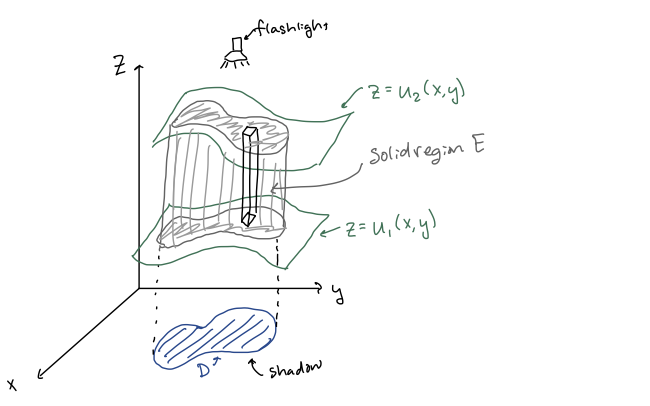
\includegraphics[width=\columnwidth]{Ch12s5-zSimple.png}

\[
\iiint_E f(x,y,z)\ dV = \iint_D \left(\int_{u_1(x,y)}^{u_2(x,y)} f(x,y,z)\ dz\right) dA
\]

%\columnbreak

\section*{x-Simple or Type 2 Solid Regions:}


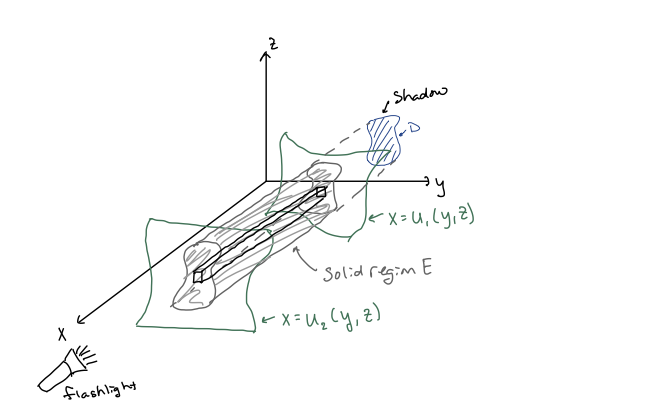
\includegraphics[width=\columnwidth]{Ch12s5-xSimple.png}

\[
\iiint_E f(x,y,z)\ dV = \iint_D \left(\int_{u_1(y,z)}^{u_2(y,z)} f(x,y,z)\ dx\right) dA
\]



%\end{multicols}
%
%\hrule
%
%\begin{multicols}{2}

\section*{y-Simple or Type 3 Solid Regions:}


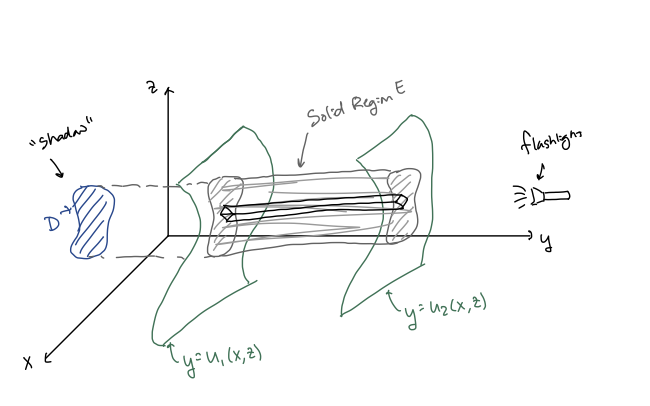
\includegraphics[width=\columnwidth]{Ch12s5-ySimple.png}

\[
\iiint_E f(x,y,z)\ dV = \iint_{D} \left( \int_{u_1(x,z)}^{u_2(x,z)} f(x,y,z)\ dy\right) dA
\]

%\columnbreak

\section*{Triple Integral Set-up Key Ideas:}

\textbf{First integrate over the ``height'' of the solid region \({E}\).}\\~\\
\textbf{Then set up a double integral over \({D}\), the ``shadow'' of the solid region in the remaining coordinate plane.}

\begin{enumerate}
\item Sketch two things:\\
Solid Region \( {E}\) \& ``Shadow'' \( {D}\)
\item Set up the iterated integral to be as easy as possible
\item The final answer should be a \textit{number},\\ so the iterated integral can have \textit{at most}:\\
inner limits: two variables\\
middle limits: one variable\\
outer limits: no variables
\end{enumerate}


%
%\end{multicols}
%
%\end{framed}

%\end{minipage}



%\section*{Examples:}


\begin{enumerate}[{Example} 1: ]
%\item Revisit ``Fun with Polar Volume'' Problem 2.
%\vfill

\item Set up a triple integral to find the volume of the solid region \( {E}\) bounded by:\\
\(z=3x^2, \qquad z=4-x^2, \qquad y=0, \qquad z+y = 6\)
\vfill

\item Set up a triple integral to find the volume of the solid region enclosed by the \textit{cylinders}\\
\(z=x^2, \qquad y=x^2\) and the \textit{planes} \(z=0, \qquad y=4\).% (Textbook 12.2.27)

\item Set up a triple integral to find the volume of the ``Ice Cream Cone'' solid region bounded above by \(x^2+y^2+z^2=4\) and below by \(x^2+y^2 = z^2\), where \(z\geq 0\).


\end{enumerate}

\pagebreak

\section*{Section 5.4 Group Work:}

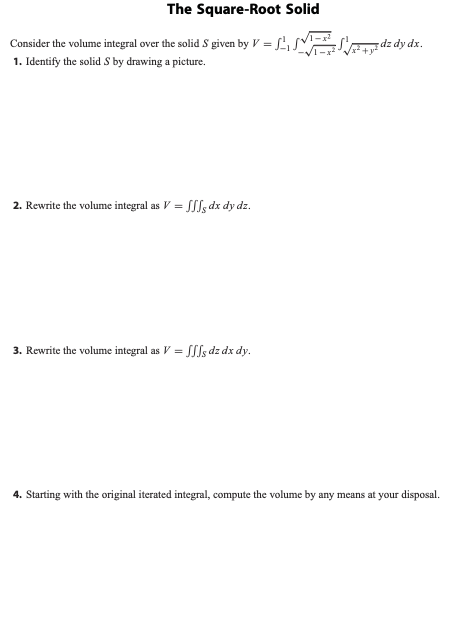
\includegraphics[height=.9\textheight]{The-Square-Root-Solid.png}



\end{document}

